\section{World Models}

\begin{frame}[plain]
  \centering
  \vspace{2.2cm}
  \Huge{\textbf{World Models}}\\[1.5em]
  \normalsize
  \textit{How generative AI can model, imagine, and predict entire environments and their dynamics.}
\end{frame}


\begin{frame}{World Models: Motivation}
  \textbf{Intuition:} a baseball batter reacts in milliseconds---action is tied to a \textbf{predictive}, action-conditioned internal model, not to slow deliberate search.
  \centering
  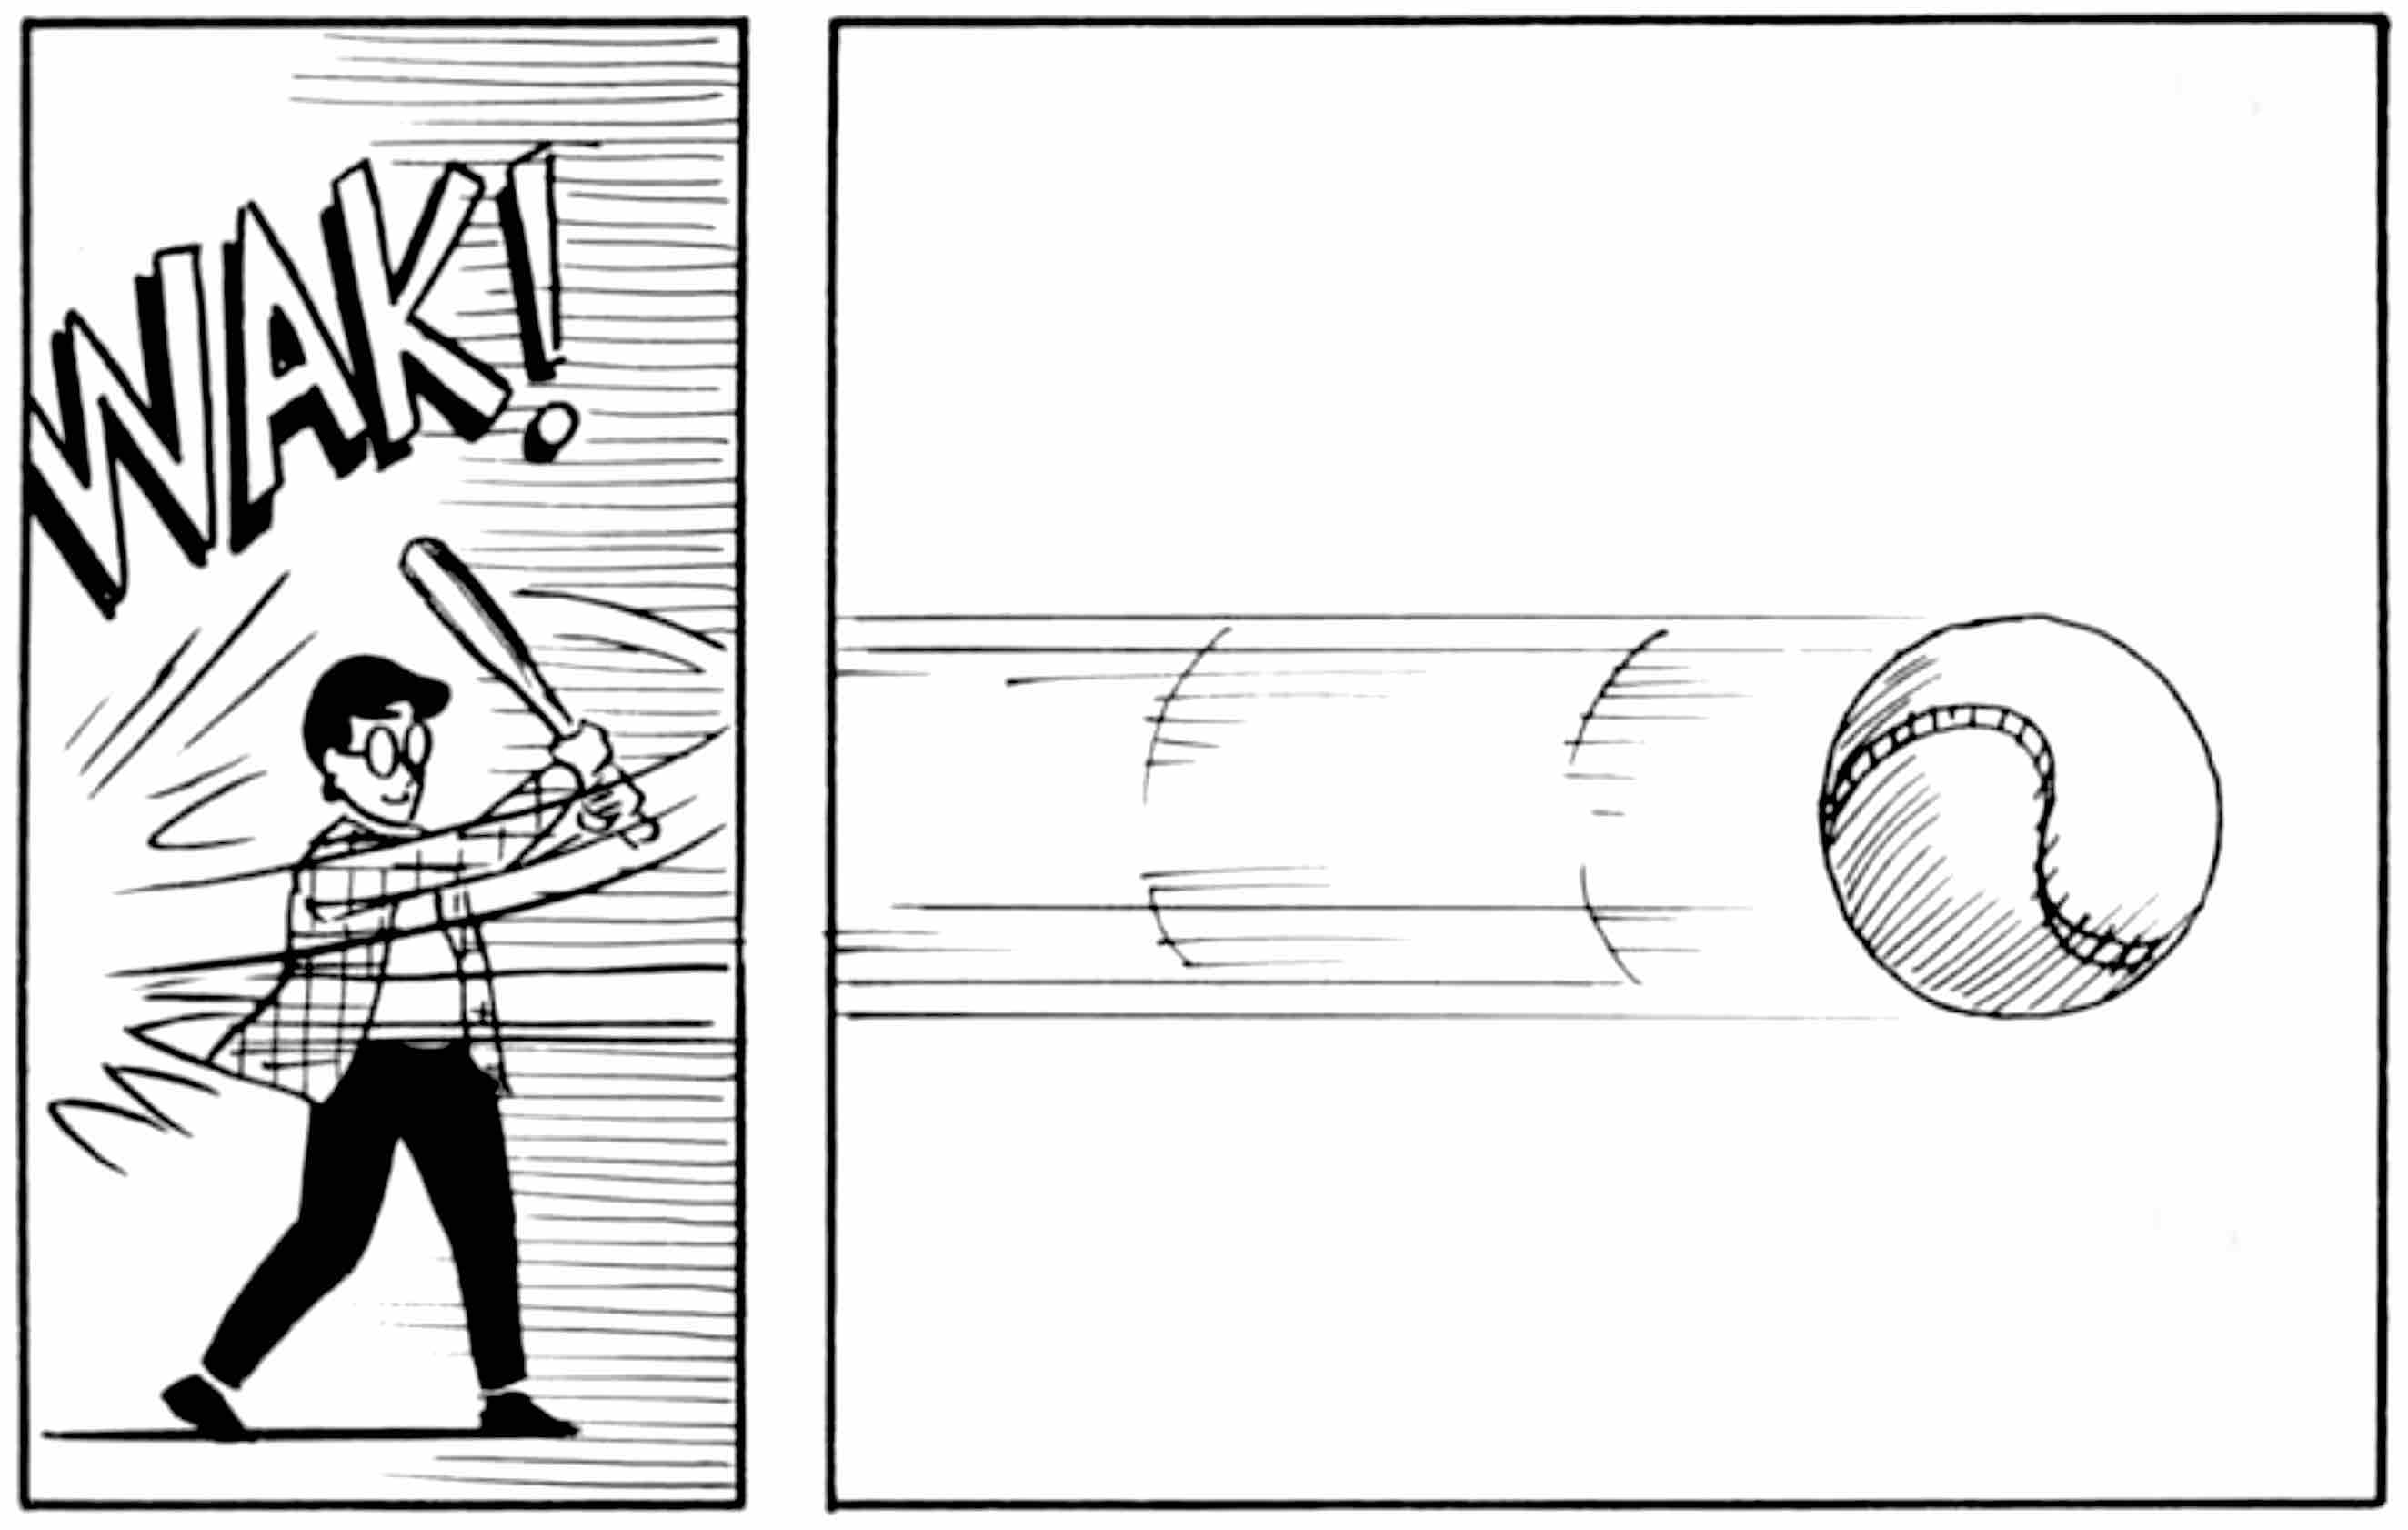
\includegraphics[width=\linewidth,height=0.72\textheight,keepaspectratio]{assets/New-Lecture_World_Models/mccloud_baseball.jpeg}\\[-0.1em]
  {\scriptsize Scott McCloud excerpt (time--space in comics).}      
\end{frame}

\begin{frame}{World Models: Motivation}
  \centering
  \vspace{0.1em}
  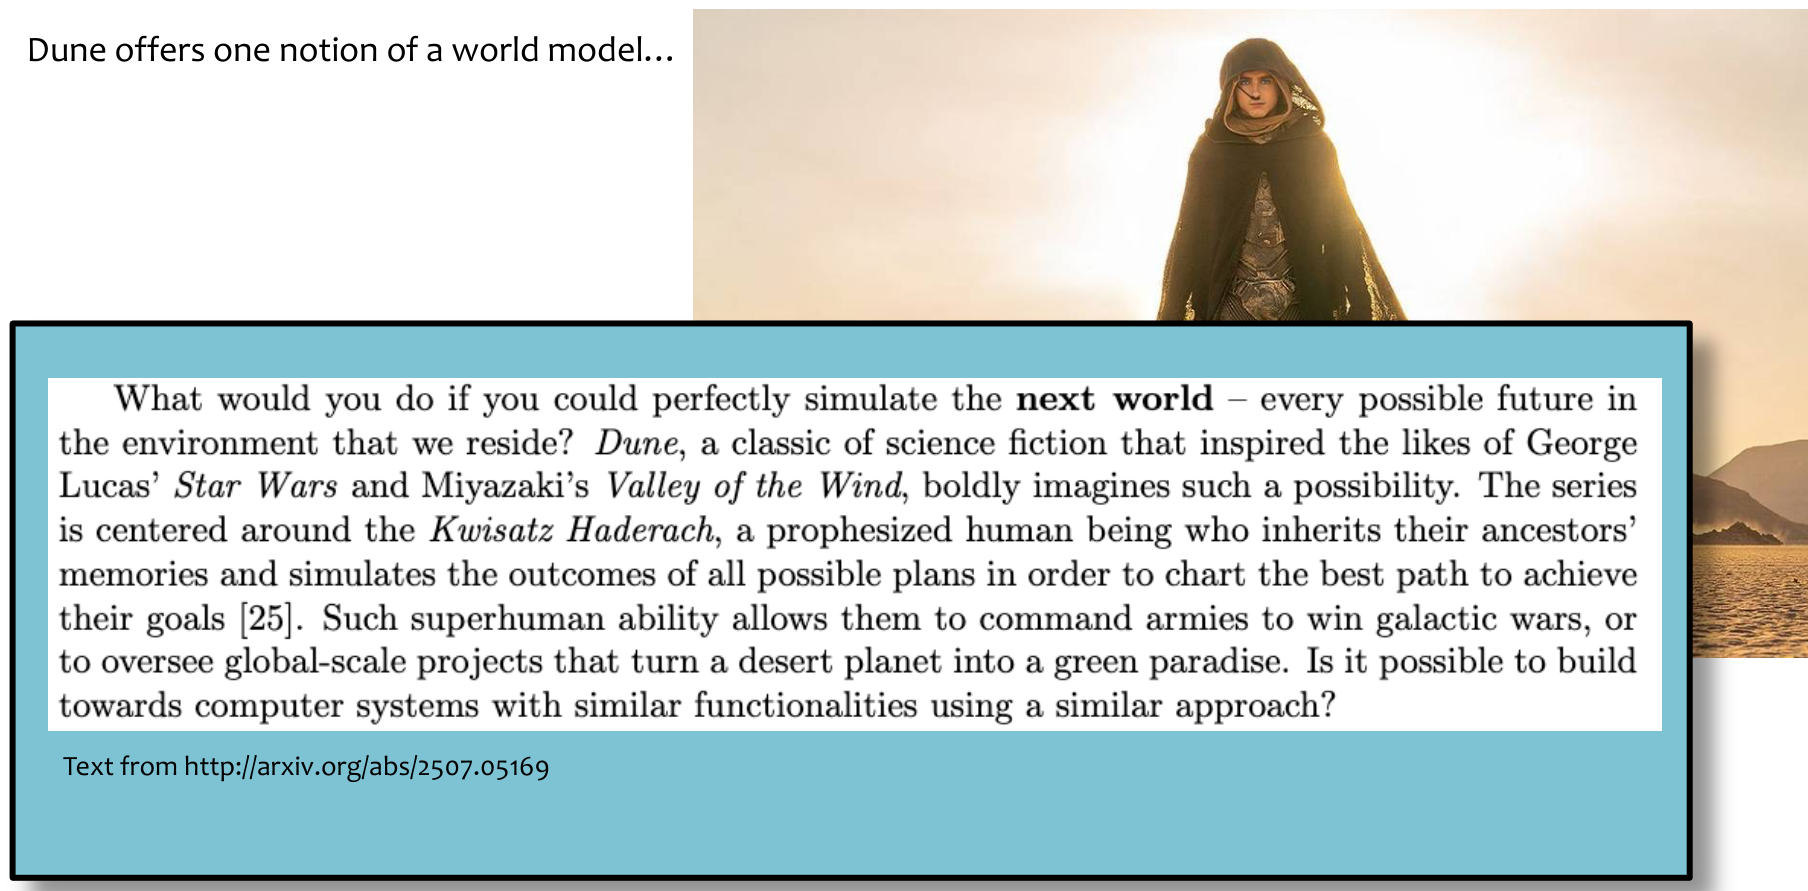
\includegraphics[width=\linewidth,height=0.88\textheight,keepaspectratio]{assets/New-Lecture_World_Models/cmu10423_lecture26_world_models_slide04.png}\\[0.32em]
  {\scriptsize CMU 10-423, Lecture 26.}
\end{frame}

\begin{frame}{World Models: Motivation}
  \centering
  \vspace{0.1em}
  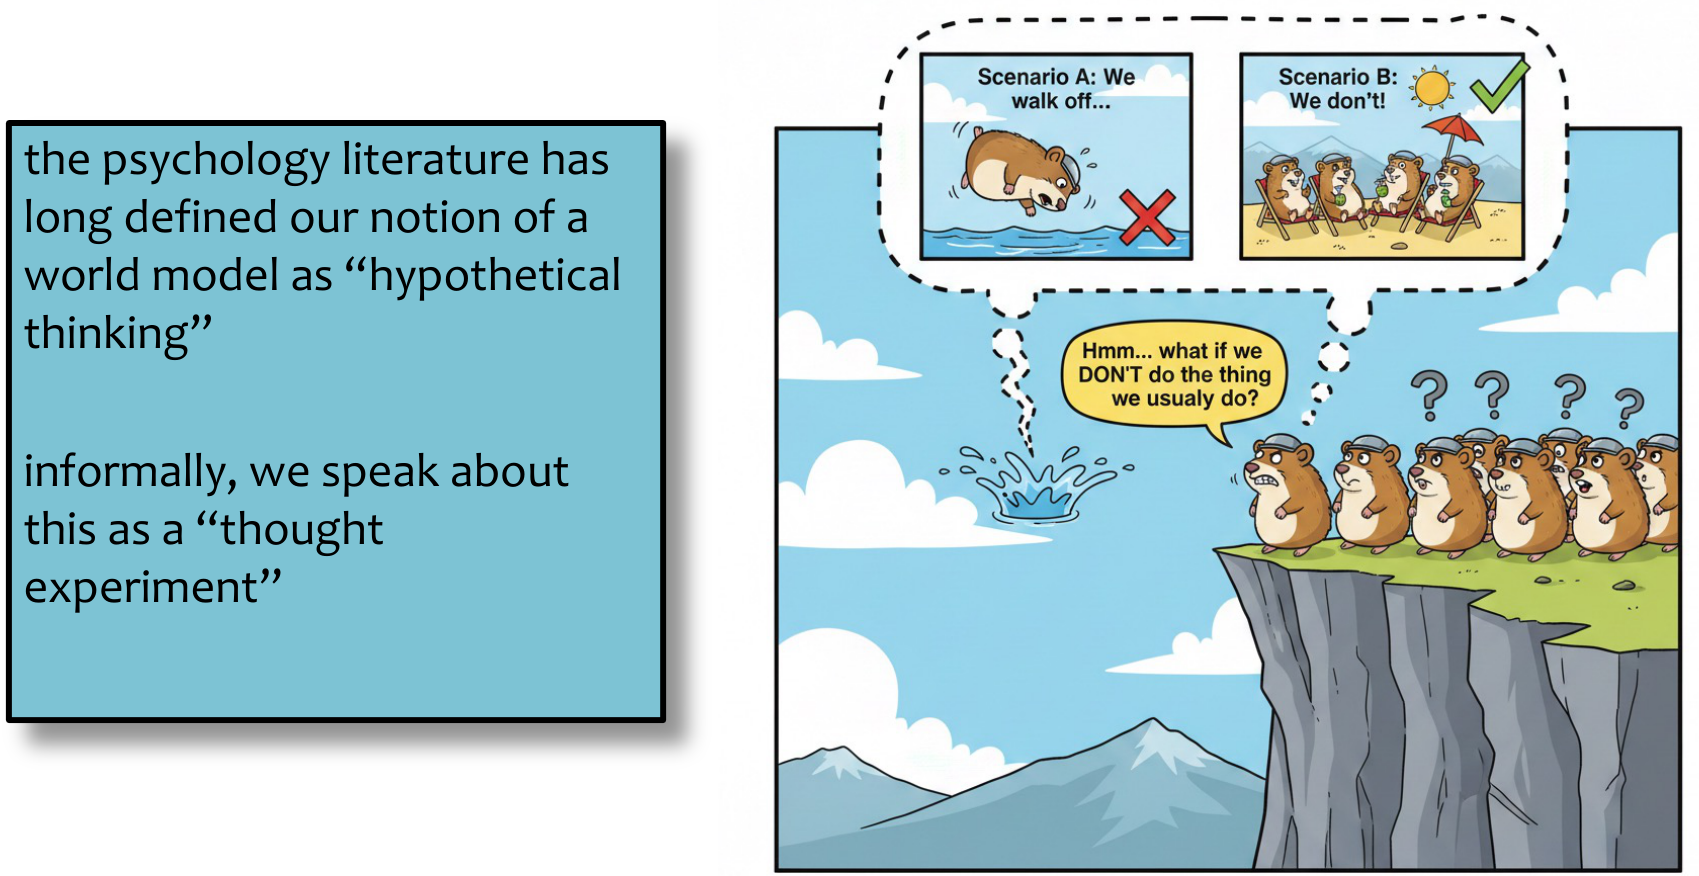
\includegraphics[width=\linewidth,height=0.88\textheight,keepaspectratio]{assets/New-Lecture_World_Models/cmu10423_lecture26_world_models_slide05.png}\\[0.32em]
  {\scriptsize CMU 10-423, Lecture 26.}
\end{frame}

\begin{frame}{World Models: Motivation}
  \begin{itemize}\itemsep0.28em
    \item[\textcolor{red}{$\blacktriangleright$}] Humans develop a mental model of the world based on what they are able to perceive with their limited senses. Our decisions and actions are based on this internal model.    
    \item[\textcolor{red}{$\blacktriangleright$}] Train a generative world model in an unsupervised way to learn a compact spatio-temporal representation of the environment.
    \item[\textcolor{red}{$\blacktriangleright$}] Use features from the world model to train a simple policy (agent) to solve the required task.
  \end{itemize}
\end{frame}

% \begin{frame}{World Models: Definition}
%   \begin{itemize}
%     \item A \textbf{world model} is a learned map that summarizes experience so we can predict (or sample) \textbf{what happens next} and sometimes \textbf{counterfactuals}: ``if I had pushed left \ldots''
%     \item An \textbf{agent} chooses actions $a_t$ and receives observations $o_t$ and rewards $r_t$. Planning and learning are easier if we can \textbf{imagine} plausible futures without acting in the real environment.
%     \item Core tension: predict \textbf{everything in pixels} (high-dimensional, noisy) vs.\ predict in a \textbf{compact latent space} (lose detail but gain stability and generalization).
%   \end{itemize}
% \end{frame}

\begin{frame}{World Models: Definition}
      % TikZ block for shaded definition box
      \begin{center}
      \begin{tikzpicture}
        \node[fill=cyan!25, rounded corners=3pt, inner sep=8pt, align=left, drop shadow] (box) {
            \begin{minipage}{0.93\columnwidth}
              \textbf{Definition:} \textit{A world model} takes a previous world state $s$ and an action $a$, and samples (or predicts) the next world state $s'$ through a distribution (or function):\\[0.6em]
              \centering
              $s' \sim p(s' \mid s, a)$
            \end{minipage}
        };
      \end{tikzpicture}
      \end{center}
\end{frame}

\begin{frame}{World Models: Definition}
  \textbf{Question:} What does a world state hold?\\[0.4em]
  \textbf{Answer:} It depends on what you're trying to model. Consider the contrast of:
  \begin{itemize}\itemsep0.24em
    \item [A)] All geopolitical entities, their leaders, and decisions they make
    \item [B)] Physical interactions in a 3D world
  \end{itemize}
\end{frame}

\begin{frame}{World Models: Overview}
    \centering
    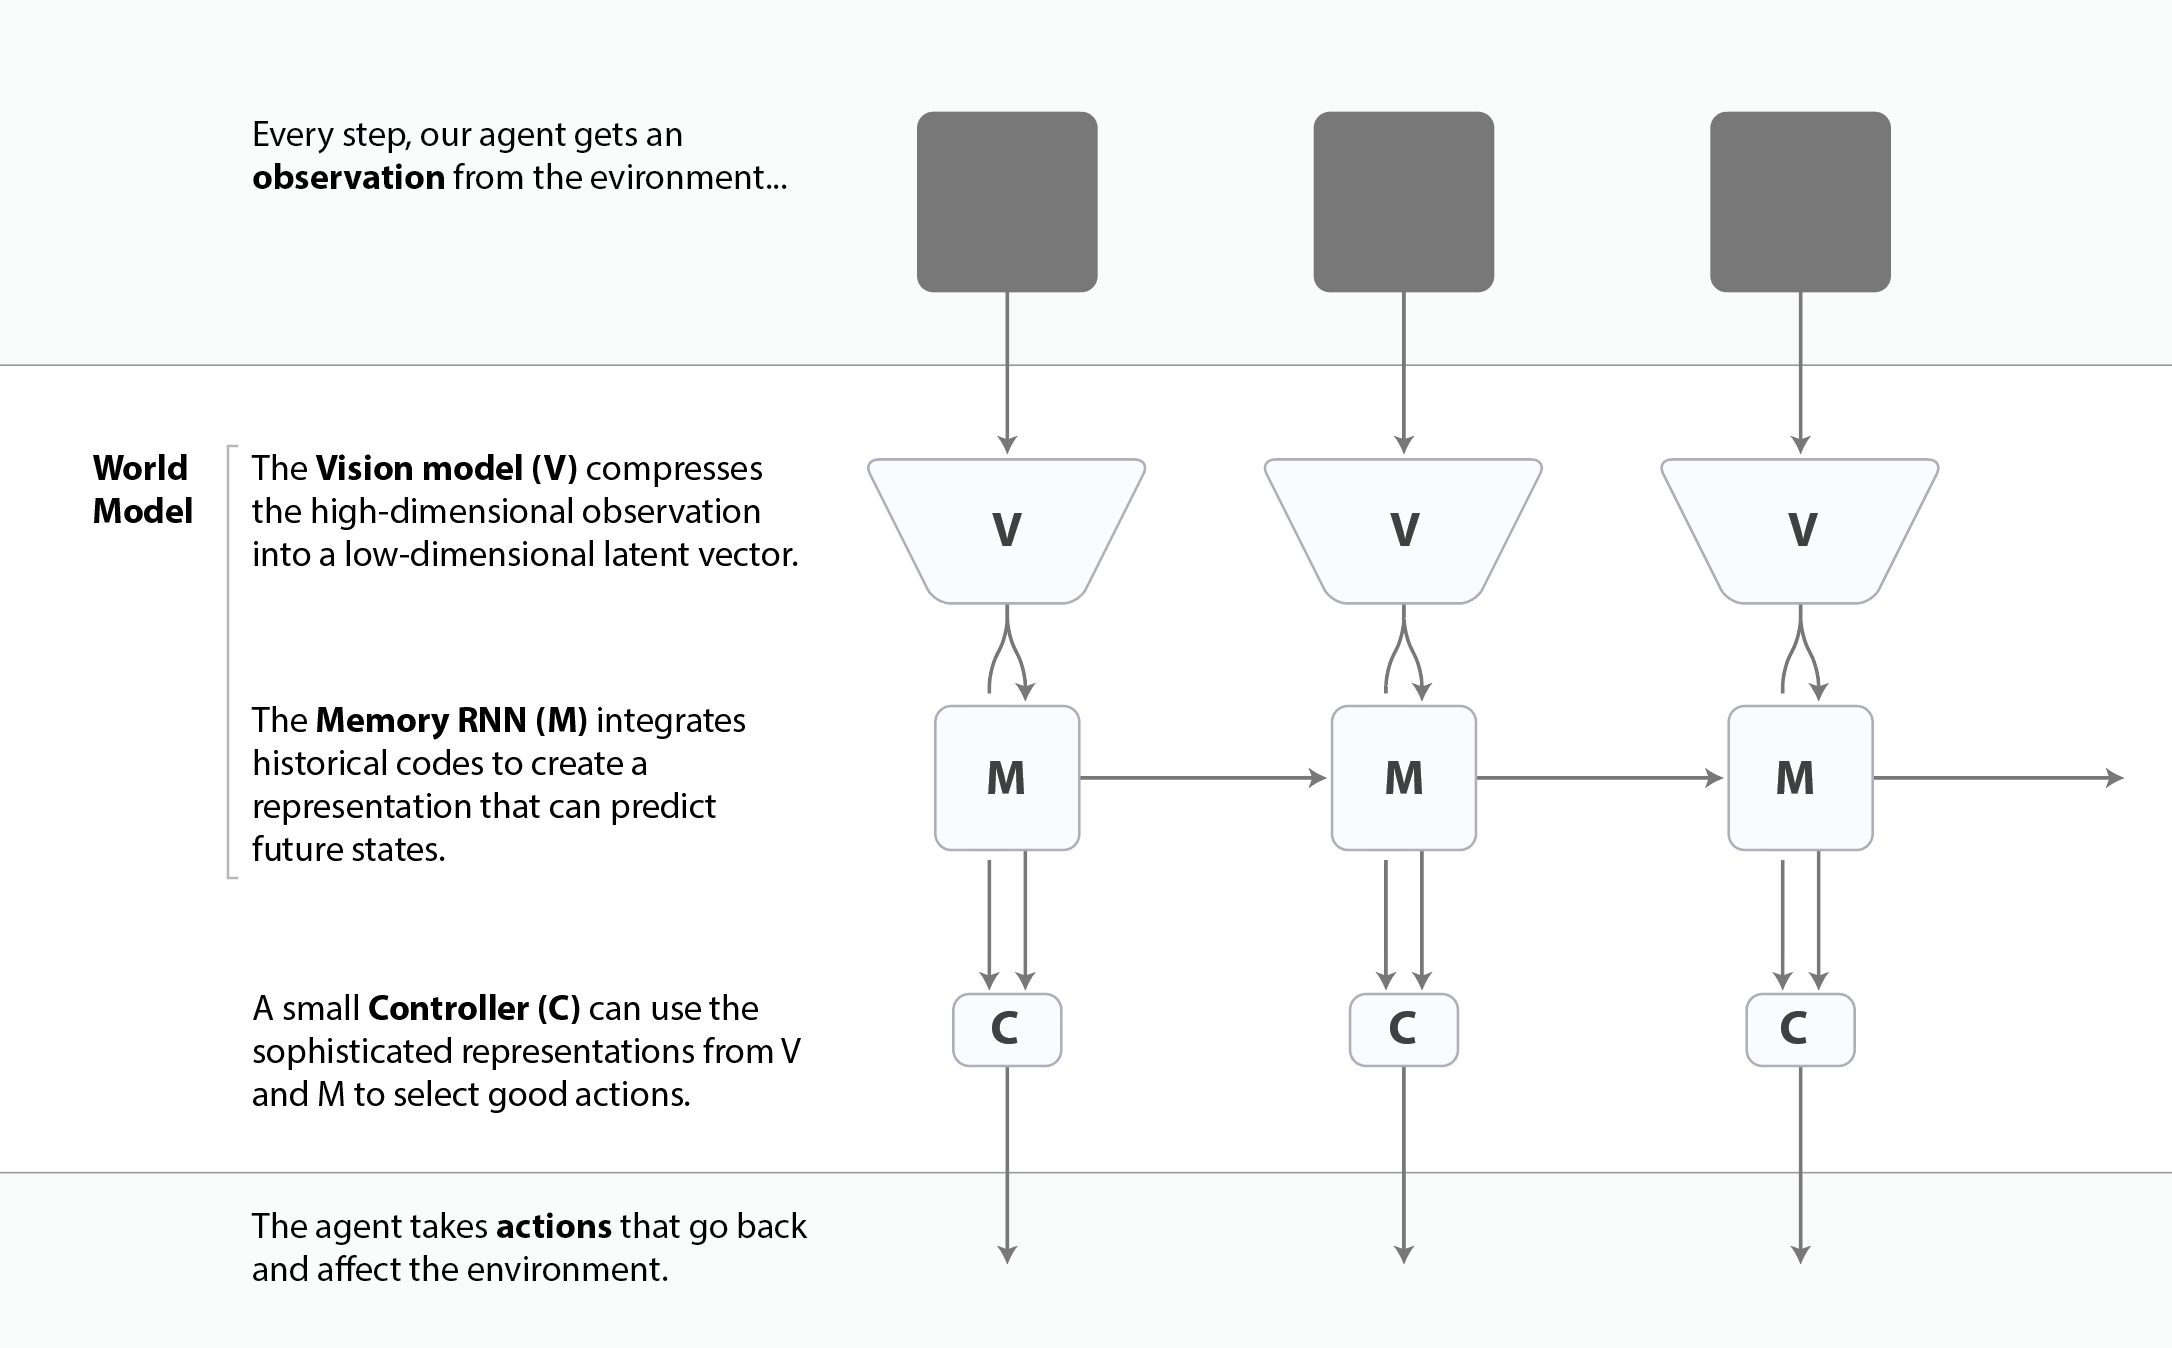
\includegraphics[width=0.95\linewidth,height=0.88\textheight,keepaspectratio]{assets/New-Lecture_World_Models/worldmodels_githubio_rollout_schematic.png}\\[0.15em]
    {\scriptsize World model overview.\\
    \textit{Source: Ha \& Schmidhuber (2018); }\href{https://arxiv.org/abs/1803.10122}{arXiv:1803.10122}.}
\end{frame}

\begin{frame}{Vision module: variational autoencoder (V)}
  \begin{columns}[T,onlytextwidth]
    \column{0.44\textwidth}
    \begin{itemize}\itemsep0.26em
      \item[\textcolor{red}{$\blacktriangleright$}] \textbf{Goal:} learn an abstract, compressed representation of each observed input frame.
      \item[\textcolor{red}{$\blacktriangleright$}] \textbf{VAE:} first stage of a two-stage sequence model---similar in spirit to modern tokenizers, but trained with classic VAE objective.
    \end{itemize}
    \column{0.54\textwidth}
    \centering
    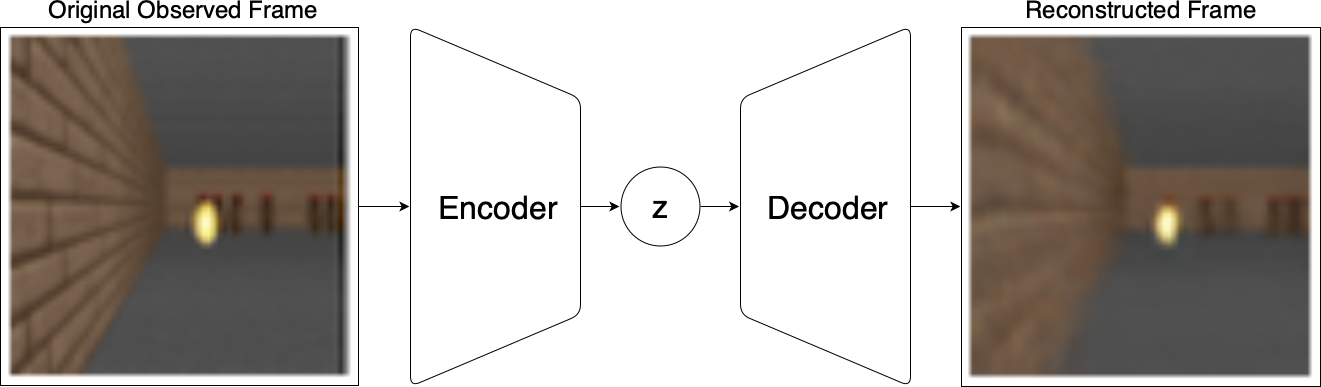
\includegraphics[width=0.95\linewidth,height=0.88\textheight,keepaspectratio]{assets/New-Lecture_World_Models/worldmodels_githubio_vae.png}\\[0.15em]
    {\scriptsize VAE diagram.\\
    \textit{Source: Ha \& Schmidhuber (2018); }\href{https://arxiv.org/abs/1803.10122}{arXiv:1803.10122}.}
  \end{columns}
\end{frame}

\begin{frame}{Memory module: Predict the future}
  \begin{columns}[T,onlytextwidth]
    \column{0.42\textwidth}
    \begin{itemize}\itemsep0.26em
      \item[\textcolor{red}{$\blacktriangleright$}] Model $p(z_{t+1} \mid z_t, a_t, h_t)$ where $z_t$ is the latent state at time $t$, $a_t$ is the action at time $t$, and $h_t$ is the hidden state at time $t$.
      \item[\textcolor{red}{$\blacktriangleright$}] adjust a temperature parameter $\tau$ to control model uncertainty
    \end{itemize}
    \column{0.56\textwidth}
    \centering
    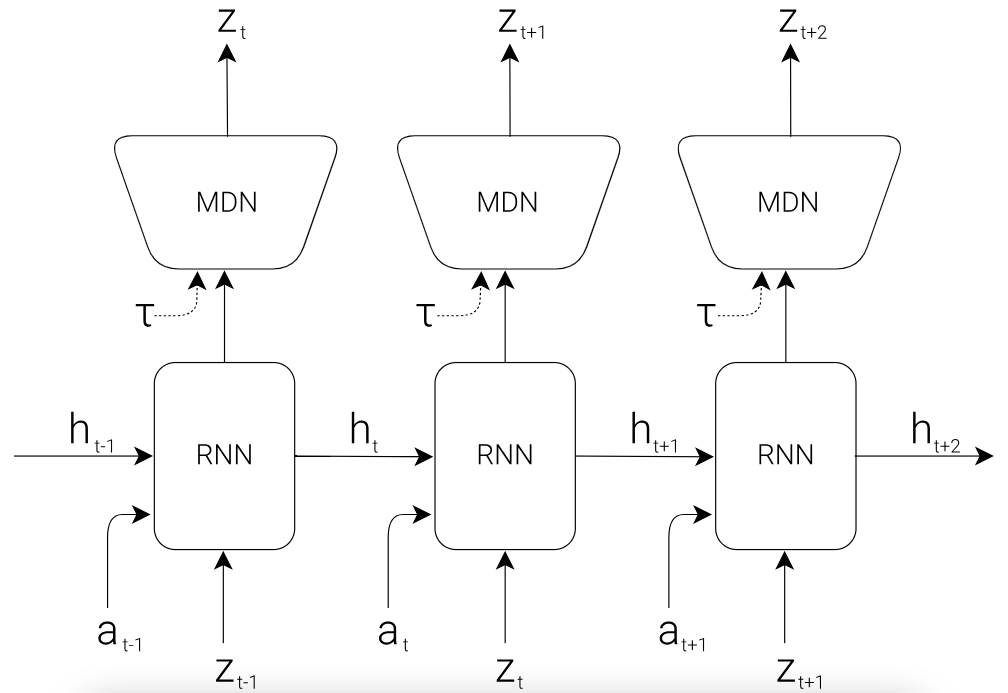
\includegraphics[width=0.95\linewidth,height=0.76\textheight,keepaspectratio]{assets/New-Lecture_World_Models/mdn_rnn_new.png}\\[0.15em]
    {\scriptsize MDN-RNN architecture.\\
    \textit{Source: Ha \& Schmidhuber (2018); }\href{https://arxiv.org/abs/1803.10122}{arXiv:1803.10122}.}
  \end{columns}
\end{frame}


\begin{frame}{Controller module: decision-making (C)}
    \begin{itemize}\itemsep0.26em
      \item[\textcolor{red}{$\blacktriangleright$}] The \textbf{Controller (C)} selects actions to maximize expected cumulative reward during agent rollout.
      \item[\textcolor{red}{$\blacktriangleright$}] Designed to be as simple and small as possible; trained \textbf{separately} from the Vision (V) and Memory (M) modules.
      \item[\textcolor{red}{$\blacktriangleright$}] Most agent complexity is thus concentrated in the world model (V and M).
      \item[\textcolor{red}{$\blacktriangleright$}] C is a \textbf{single-layer linear} model that maps the latent vector $z_t$ and RNN hidden state $h_t$ directly to the action $a_t$ at each time step:
    \end{itemize}
    \vspace{0.7em}
    {\small
    \[
      a_t = W_c [z_t; h_t] + b_c
    \]
    }
    \begin{itemize}\itemsep0.15em
      \item[\textcolor{red}{$\blacktriangleright$}] Here, $W_c$ and $b_c$ are the weight matrix and bias; $[z_t; h_t]$ is the concatenated latent and memory state.
      \item[\textcolor{red}{$\blacktriangleright$}] Output vector $a_t$ is the action taken by the agent.
    \end{itemize}
    % Optionally: say evolved with CMA-ES, not trained end-to-end.
\end{frame}

\begin{frame}{World model: Putting Everything Together}
  \centering
  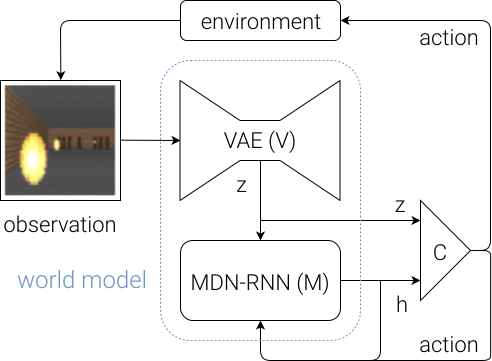
\includegraphics[width=\linewidth,height=0.78\textheight,keepaspectratio]{assets/New-Lecture_World_Models/world_model_schematic_downloads.png}\\[0.28em]
  {\scriptsize Agent-environment flow (observation $\rightarrow$ $z_t$, RNN state $h_t$, action $a_t$, next step).\\
  \textit{Source: Ha \& Schmidhuber (2018); }\href{https://arxiv.org/abs/1803.10122}{arXiv:1803.10122}.}
\end{frame}


% \begin{frame}[plain]
%   \centering
%   \vspace{0.1em}
%   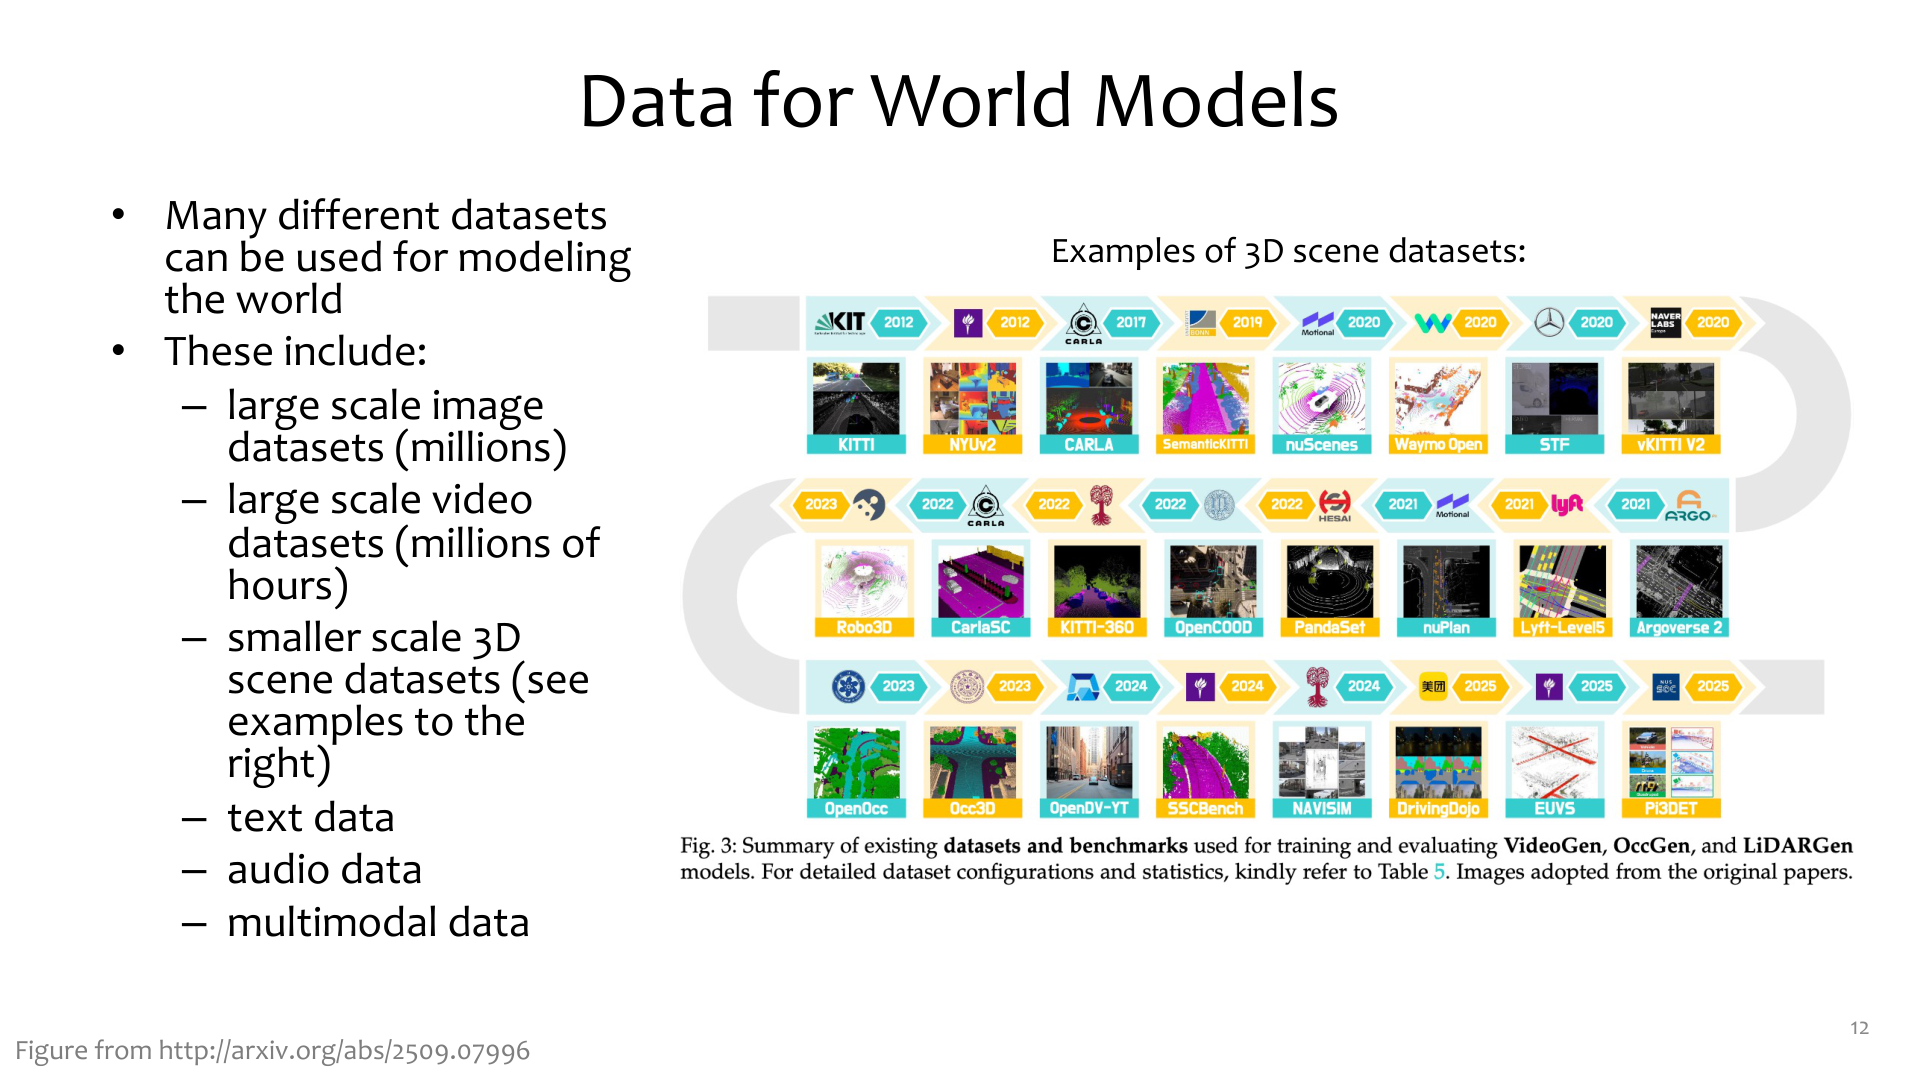
\includegraphics[width=\linewidth,height=0.88\textheight,keepaspectratio]{assets/New-Lecture_World_Models/cmu10423_lecture26_world_models_slide08.png}\\[0.32em]
%   {\scriptsize Same deck --- slide 8 (data modalities: image/video/3D/text/audio/multimodal).}
% \end{frame}

% \begin{frame}[plain]
%   \centering
%   \vspace{0.1em}
%   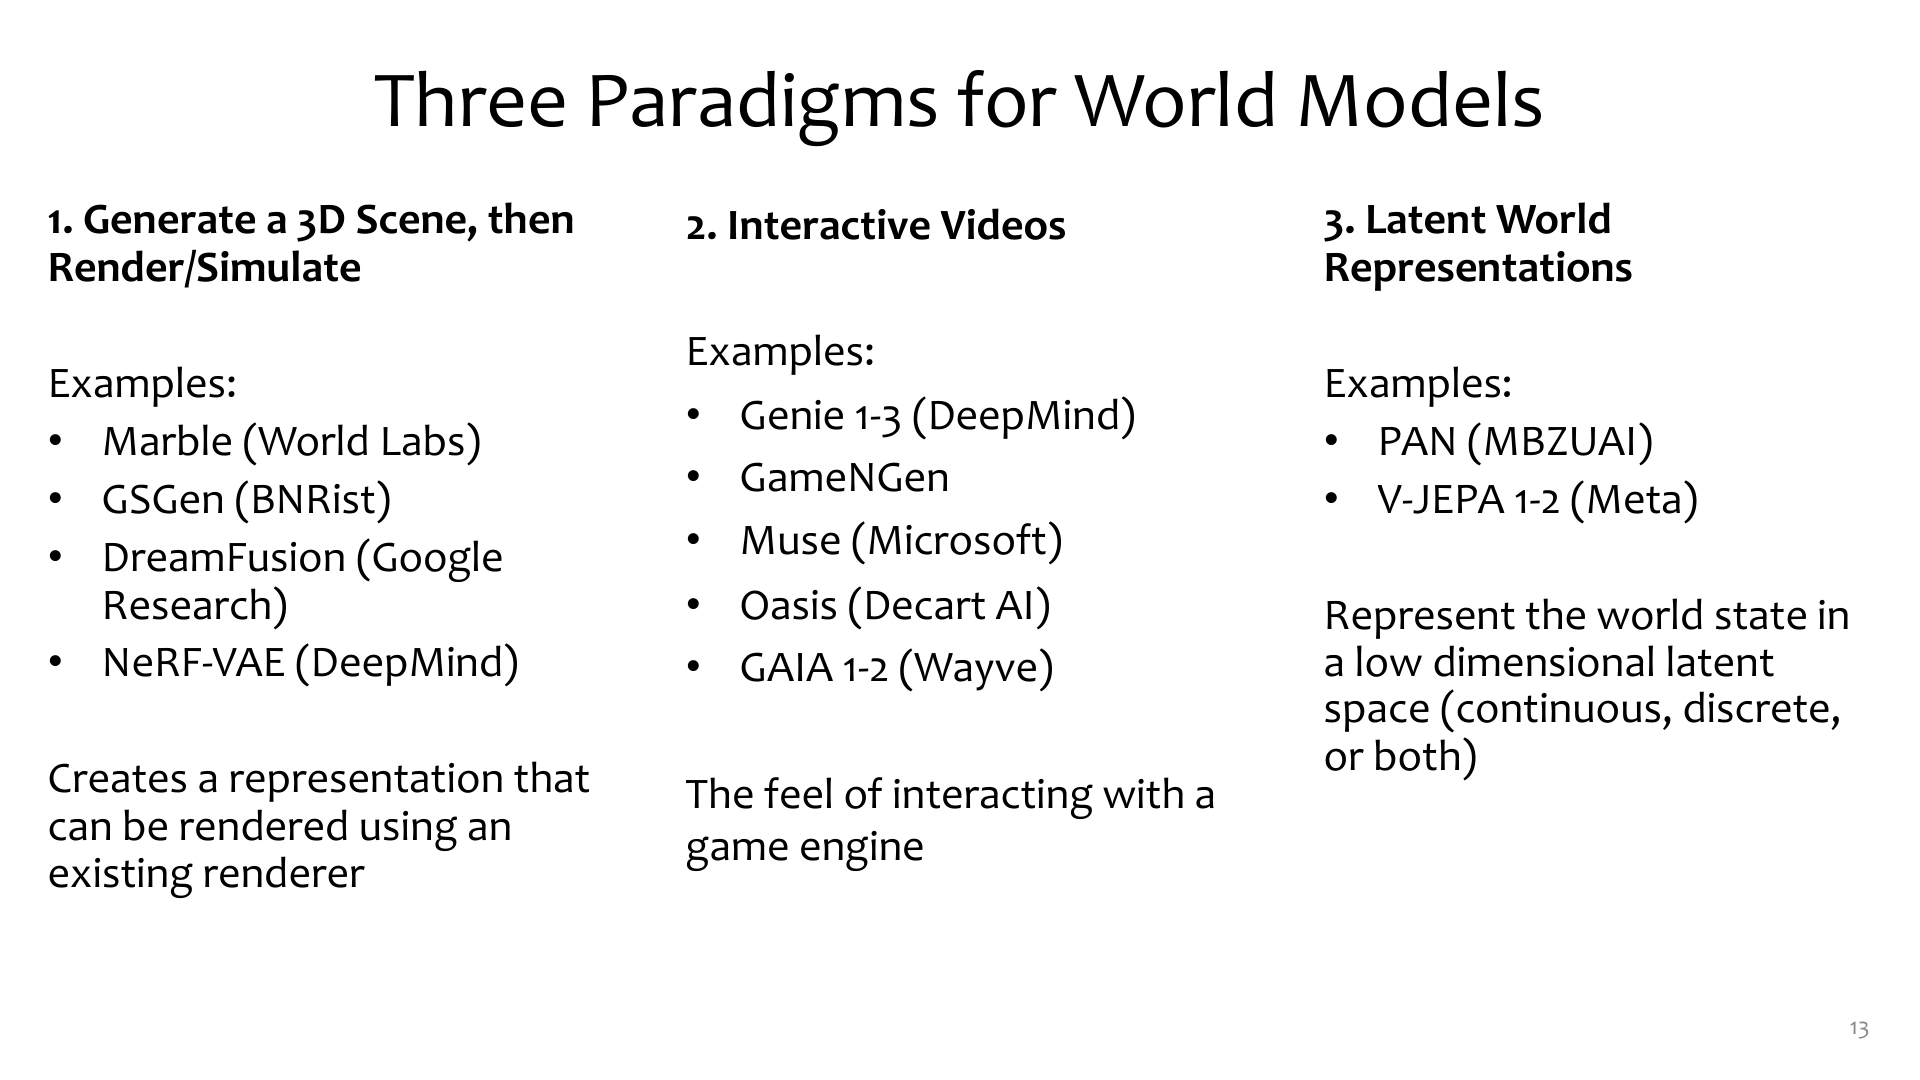
\includegraphics[width=\linewidth,height=0.88\textheight,keepaspectratio]{assets/New-Lecture_World_Models/cmu10423_lecture26_world_models_slide09.png}\\[0.32em]
%   {\scriptsize Same deck --- slide 9 (three paradigms: 3D scene+render; interactive video; latent representations).}
% \end{frame}
